\documentclass[english]{scrartcl}
\usepackage[T1]{fontenc}
\usepackage{listings}
\usepackage{hyperref}
\usepackage{graphicx}
\usepackage{color}
\usepackage{soul}
\usepackage{seqsplit}
\usepackage{multirow}
\usepackage{enumitem}
\usepackage{graphicx}
\usepackage{float}
\usepackage{amsmath}
\begin{document}

\section*{Task 6.1}
Development of the state is visualised in Figure \ref{fig:6-1}.

\begin{figure}[h]
\centering
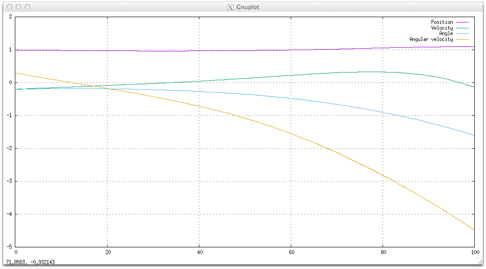
\includegraphics{./6-1}
\caption{State development with F=0}
\label{fig:6-1}
\end{figure}

\section*{Task 6.2}
Development of the state for parameters $k_{1} = -1, k_{2} = 3, k_{3} = -1, k_{4} = 2$ is visualised in Figure \ref{fig:6-2}.

\begin{figure}[h]
\centering
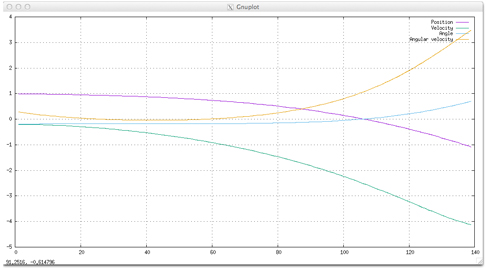
\includegraphics{./6-2}
\caption{State development with $F=min(20,max(-20,k_{1}*position+k_{2}*velocity+k_{3}*angle+k_{4}*angular-velocity))$}
\label{fig:6-2}
\end{figure}

\section*{Task 6.3}
The learning process was held for 5000 iterations with $\epsilon=0.8$ and $\alpha=0.01$. The learning process is visualised in Figure \ref{fig:6-3}.

\begin{figure}[h]
\centering
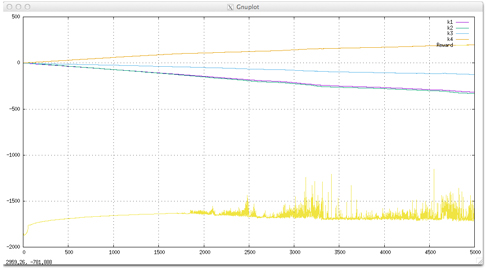
\includegraphics{./6-3}
\caption{Learning process}
\label{fig:6-3}
\end{figure}

It can be seen, that from some moment learning process stops improvement of the reward, but from next oscillations of the reward one can be chosen as the best: -994. That reward is got for parameters $k_{1}=-485.44374999999945, k_{2}=-513.5300000000018, k_{3}=-230.34125000000085, k_{4}=281.4124999999998$ and the length of the episode is 646 steps and development of states for these values is visualised in Figure \ref{fig:6-3-the-best}.

\begin{figure}[h]
\centering
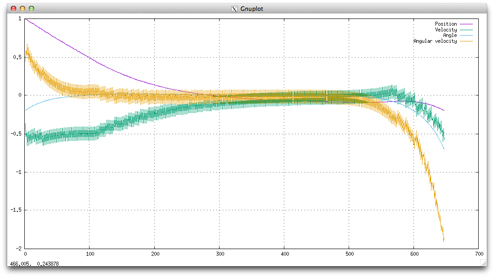
\includegraphics{./6-3-the-best}
\caption{State development for best parameters}
\label{fig:6-3-the-best}
\end{figure}

\end{document}

